\documentclass[11pt,a4paper]{article}

\usepackage[utf8]{inputenc}
\usepackage[margin=1.0in]{geometry}
\usepackage{amsmath,amssymb,amsfonts,amsthm}
\usepackage{graphicx}
\usepackage{subcaption}
\usepackage{booktabs}
\usepackage{multirow}
\usepackage{array}
\usepackage{hyperref}
\usepackage[natbibapa]{apacite}
\usepackage{setspace}
\usepackage{abstract}
\usepackage{makecell}
\usepackage{algorithm}
\usepackage{algpseudocode}
\usepackage{url}

\newtheorem{proposition}{Proposition}
\newtheorem{proof_prop}{Proof}

\hypersetup{
    colorlinks=true,
    linkcolor=black,
    citecolor=black,
    urlcolor=black
}

\onehalfspacing

\title{\textbf{Institutional Portfolio Construction under Cardinality Friction:\\A Diversity-Aware Adaptive Metaheuristic Framework}}

\author{
    \textbf{Atishaya Jain}\textsuperscript{1},
    \textbf{Karan Jangra}\textsuperscript{1},
    \textbf{Vaibhav Pacherwal}\textsuperscript{1}\\
    \small \textsuperscript{1}Department of Computer Science and Engineering,\\
    \small Netaji Subhas University of Technology (NSUT), New Delhi, India\\
    \small \texttt{atishaya.jain.ug23@nsut.ac.in},
    \texttt{karan.jangra.ug23@nsut.ac.in},
    \texttt{vaibhav.pacherwal.ug23@nsut.ac.in}
}

\date{\today}

\begin{document}

\maketitle

\begin{abstract}
With large equity universes, institutional portfolio optimisation faces serious non convex allocation constraints, high risk of parameter estimation, and early algorithmic stagnation. Realistic cardinality limits ($K=30$) or asset exposure caps ($W_{\max}=20\%$) on individual assets impose severe structural limits on traditional analytical solvers, such as Markowitz quadratic programming. Since candidates cannot allocate their risks incrementally, dimension-independent population-based metaheuristics are unable to navigate nondifferentiable landscapes and tend to become stuck in local minima of risk, which causes a diversity collapse.

This paper aims at presenting a diversity-aware and feasibility-preserving optimization framework called \textbf{AOBL-SOS} (Adaptive Opposition-Based Learning Symbiotic Organisms Search) for constructing non-convex portfolio. Empirical validation is performed on a point in time equity universe in a standardized manner, expanding the walk forward testing horizon, covering 2018–2024, that is represented by seven different out of sample testing windows, eliminating the survivorship bias. When executed with large-scale $AUM = \$100\text{M}$ Almgren-Chriss friction for each rebalancing, AOBL-SOS significantly outperforms the baseline metaheuristics in terms of out-of-sample risk-adjusted performance:OS Sharpe ratio 0.841, CAGR 17.27\%, vs. OS Sharpe 0.733 for SOS, OS Sharpe 0.734 for PSO, OS Sharpe 0.727 for GA, OS Sharpe 0.609 for DE. A new, 6-variant walk-forward study also shows that incorporating a drawdown penalization based on the path followed with an adaptive opposition based on the centroid means a superior risk-adjusted allocation. Moreover, real-world out-of-sample Sharpe ratio is above trial-inflation hurdles, at the same time both inter-grid selection variability and a CSCV Probability of Backtest Overfitting $\text{PBO} = 0.6998$ ($69.98\% \times 6$ confidence interval) are confirmed, respectively. Carhart 4-factor multi-factor regressions demonstrate that performance is driven by systematic market beta ($\beta_{\text{MKT}} = 0.924, t=56.94$), value ($\beta_{\text{HML}} = 0.291, t=10.23$), and momentum factor exposure ($\beta_{\text{MOM}} = 0.638, t=19.96$).
\end{abstract}

\noindent \textbf{Keywords:} Portfolio Optimization, Cardinality Constraints, AOBL, SOS, Almgren-Chriss Execution, Walk-Forward Analysis, Backtest Overfitting.

\section{Introduction}

Modern quantitative asset allocation is an exercise in navigating highly constrained non-convex mathematical spaces The portfolio selection is based on Markowitz's \cite{markowitz1952} mean-variance framework. Two fundamental bottlenecks that limit the use of portfolio selection in practice by institutions are: (1) extreme sensitivity to input covariance and return estimates \cite{michaud1989} and (2) the requirement of continuous, twice-differentiable constraint sets \cite{black1992}. In some cases, institutional mandates place strict bounds on operations such as exact cardinality constraints ($\|\mathbf{w}\|_0 = K = 30$) that limit transaction overhead, or position exposure caps ($w_i \le 20\%$) that guaranty diversification. This renders the optimization problem an NP-hard Mixed-Integer Nonlinear Programming (MINLP) problem \cite{chang2000}.

Typical commercial solvers solve cardinality bounds using convex relaxation or greedy rounding heuristics that often result in poor suboptimal weights which contradict operational requirements or fail in out-of-sample market stress testing \cite{bertsimas1999, fabozzi2007}. On the contrary, simple diversification strategies like the equal weighting $1/N$ strategy often beat advanced optimization algorithms on account of the presence of estimation error in the sample covariance matrix \cite{demiguel2009}. Metaheuristic techniques based on population search techniques, e.g., Genetic Algorithms (GA) \cite{holland1992}, Particle Swarm Optimization (PSO) \cite{kennedy1995}, and Differential Evolution (DE) \cite{storn1997}, show great promise for navigating through non-convex financial landscapes \cite{gilli2001, cheng2014}. However, conventional metaheuristics have serious drawbacks when dealing with high dimensional financial problems due to premature convergence of the candidate solutions in the early iterations of the search process \cite{bailey2014}.

Four main contributions overcome both the premature convergence and the handling of constraints in this study:

\begin{enumerate}

\item \textbf{Feasibility-Preserving Simplex Encoding:} The construction of a continuous latent solution encoding $\mathbf{x} \in \mathbb{R}^n$ is coupled with a deterministic mapping of the active subset $(\mathbf{S}(\mathbf{x}), \boldsymbol{\theta}(\mathbf{x}))$ to transmit and directly constrain the unrestricted optimization parameters to the capped probability simplex, respecting their cardinality and forming feasible individuals in population and any subsequently discovered \textit{ex nihilo}. We forgo repair mechanisms.
 \item \textbf{Centroid-Based Adaptive Opposition Mechanism:} Departing from uniform permutation opposition \cite{tizhoosh2005}, we leverage an opposition operator \cite{fomin2011} that operates on the mean of individuals with respect to the mean \textit{center of mass} of stagnant allocations in population $\mathbf{c}$, $\mathbf{x}_{\text{opp}} = \mathbf{c} + \gamma(\mathbf{c} - \mathbf{x})$. Factor $\gamma$ increases in real time response to population diversity decay.
 \item \textbf{Survivorship-Bias-Free Walk-Forward Protocol:} A temporal filtering of investable universe at each decision point, based solely on historical prior data availability and constructing a new "universe", using seven distinct walk-forward windows of decreasing size over periods Jan 1, 2018--Dec 31, 2024, where each step begins on the last decision date and employs solely data known prior to that point, has removed survivorship and out-of-sample testing bias.
 \item \textbf{Institutional Execution \& Overfitting Validation:} We explore the robustness of our model under typical market trading environments including the Almgren-Chriss square-root model of market impact \cite{almgren2001}. Performance is also validated against a raft of standard overfitting metrics, including Combinatorial Symmetric Cross-Validation (CSCV) \cite{bailey2017}, Carhart 4-factor risk factor multi-factor regressions, varying asset universe size ($10\text{M}-5\text{B}$), and VIX market regime conditions.

\end{enumerate}

\section{Literature Review}

\subsection{The Cardinality Bottleneck \& Non-Convex Optimization}
The cardinality constraint $\|w\|_0\le K$ limits the portfolio to have at most $K$ active assets from an investable universe of $n$ stocks. Exact solutions require \cite{woodside2011} to solve a combinatorial choice of $\binom{n}{K}$ continuous sub-problems. Exact MINLP branch-and-bound algorithms are computationally intractable for institutional equity universes (e.g., $n>100$) \cite{gao2013}. $L_1$-regularization and sparse portfolio estimators \cite{brodie2009} induce sparsity but cannot impose exact cardinality bounds $K$ or upper position bounds $W_{\max}$ simultaneously without distorting the return-risk objective function.

\subsection{Metaheuristics \& Diversity Collapse}
Stochastic population based metaheuristics avoid differentiability constraints by directly evaluating candidate allocation using objective fitness functions \citep{maringer2005, corne2012}. The biological interactions (mutualism, commensalism, parasitism) are modeled using a model called Symbiotic Organisms Search (SOS) \cite{cheng2014} which doesn't require tuning parameters that are algorithm specific. In the case of financial spaces of high dimension, however, the population vectors quickly converge along the most important eigenvectors of the covariance matrix, such that the population diversity $D_t$ decreases exponentially. Opposition Based Learning (OBL) \cite{tizhoosh2005, rahnamayan2008} speeds up search by checking the opposite candidate vectors. But classical OBL operators use static search space boundaries: $lb + ub - x$ which is not applicable on probability simplices. In this paper, the limitation is overcome by creating adaptive opposition based on the centroid.

\subsection{Path-Dependent Downside Risk Objectives}
Variance measures dispersion in a symmetrical way, which is problematic at crisis events like the 2008 Global Financial Crisis and the 2020 COVID-19 crash. Tail risk measures like Conditional Value-at-Risk (CVaR) \cite{rockafellar2000} and Sortino ratios \cite{sortino1994} enhance the downside analysis of risk. But MDD is a path-dependent measure of the greatest peak-to-trough loss of capital (deficit) \cite{magdon2004, chekhlov2005}. Forcing optimizers to avoid allocations that fit the fragile "sharpe" definition in the metaheuristic formulations of fitness will force drawdown penalties into the formulation.

\subsection{Execution Shortfall \& Backtest Overfitting}
Theoretical alpha is often wiped out during the actual trading process because of friction from bid-ask price spread and lack of impact on the price \cite{roll1984, amihud2002, hasbrouck2009}. The Almgren-Chriss square-root model \cite{almgren2001} measures some non-linear execution costs of block orders as a function of Average Daily Volume (ADV). Also, selecting a strategy that has a high-dimensionality introduces high selection bias. Bailey and López de Prado \cite{bailey2014} and Bailey et al. \cite{bailey2017} prove that the CSCV and the DSR are both quantifications of backtest overfitting that adjust out-of-sample performance for the number of explore configurations.

\section{Methodology and Optimization Framework}

\subsection{Problem Formulation \& Institutional Constraints}
Consider an investable universe of $n$ assets with daily return vector $\mathbf{r}_t \in \mathbb{R}^n$. Let $\mathbf{w} = [w_1, w_2, \dots, w_n]^T \in \mathbb{R}^n$ represent portfolio weights. The institutional portfolio selection problem is formulated as a loss minimization task:
\begin{equation}
\min_{\mathbf{w}} \quad g(\mathbf{w}) = -\text{SR}(\mathbf{w}) + \lambda \cdot |\text{MDD}(\mathbf{w})|
\end{equation}
subject to strict institutional constraints:
\begin{align}
\sum_{i=1}^n w_i = 1, \quad & \text{(Budget Constraint)} \\
w_i \ge 0, \quad \forall i \in \{1, \dots, n\}, \quad & \text{(Long-Only Constraint)} \\
\|\mathbf{w}\|_0 = \sum_{i=1}^n \mathbb{I}(w_i > 0) = K, \quad & \text{(Cardinality Constraint)} \\
w_i \le W_{\max}, \quad \forall i \in \{1, \dots, n\}, \quad & \text{(Position Exposure Cap)}
\end{align}
where $\text{SR}(\mathbf{w})$ is the annualized Sharpe ratio, $\text{MDD}(\mathbf{w}) = \min_{t} \left( \frac{V_t - \max_{\tau \le t} V_\tau}{\max_{\tau \le t} V_\tau} \right)$ is the peak-to-trough maximum drawdown of portfolio value $V_t$, and $\lambda \ge 0$ is the drawdown penalty coefficient.

\subsection{Feasibility-Preserving Solution Encoding & Mapping}
To optimize over non-convex portfolio landscapes without post-hoc repair heuristics, candidate allocations are represented as continuous organisms $\mathbf{x} \in \mathbb{R}^n$ over the full cross-sectional asset universe $n$. A two-stage transformation operator $\mathcal{M}: \mathbb{R}^n \to \Delta^{n-1}(W_{\max})$ maps continuous vectors into strictly feasible portfolio allocations:
\begin{enumerate}
    \item \textbf{Binary Selection & Active Subset Identification:} The $K$ largest components of $\mathbf{x}$ define the binary active asset selection mask $\mathbf{S} \in \{0, 1\}^n$ where $\|\mathbf{S}\|_0 = K$ (with $K=30$). Unselected assets $i \notin \text{top-}K(\mathbf{x})$ receive weight $w_i = 0$. Because individual position caps ($W_{\max}=20\%$) require at least $\lceil 1/W_{\max} \rceil = 5$ assets to satisfy $\sum w_i = 1$, setting $K=30$ enforces exact cardinality while maximizing risk-adjusted diversification.
    \item \textbf{Capped Simplex Water-Filling Projection:} The active latent vector $\boldsymbol{\theta} = \mathbf{x}_{\text{top-}K} \in \mathbb{R}^K$ is transformed onto the probability simplex via a softmax mapping:
    \begin{equation}
    \tilde{w}_i = \frac{\exp(\theta_i)}{\sum_{j=1}^K \exp(\theta_j)}, \quad i \in \{1, \dots, K\}
    \end{equation}
    If any entry exceeds $W_{\max}$, excess weight is iteratively redistributed across uncapped active assets:
    \begin{equation}
    w_i^{(k+1)} = \min\left(W_{\max}, \, w_i^{(k)} + \Delta \cdot \frac{w_i^{(k)}}{\sum_{j \notin \mathcal{C}} w_j^{(k)}}\right)
    \end{equation}
    where $\mathcal{C} = \{j \mid w_j = W_{\max}\}$ is the set of capped assets and $\Delta = \sum_{j \in \mathcal{C}} (w_j^{(k)} - W_{\max})$ is the excess weight to redistribute. (See Appendix A for formal proof of feasibility preservation).
\end{enumerate}

\subsection{Symbiotic Organisms Search (SOS) on Latent Representation}
SOS \cite{cheng2014} is a parameter-free metaheuristic that simulates biological interactions among organisms in an ecosystem $\mathbf{X} = \{\mathbf{x}_1, \mathbf{x}_2, \dots, \mathbf{x}_N\}$ in continuous space $\mathbb{R}^n$. All metaheuristic phase updates (Mutualism, Commensalism, Parasitism) operate directly on continuous decision vectors $\mathbf{x}_i \in \mathbb{R}^n$, providing smooth gradient-free exploration while $\mathcal{M}(\mathbf{x}_i)$ guarantees strict feasibility at every loss evaluation $g(\mathcal{M}(\mathbf{x}_i))$. Each iteration $t$ executes three sequential phases:

\subsubsection{Mutualism Phase}
Organism $\mathbf{x}_i$ interacts with a randomly selected organism $\mathbf{x}_j$ ($j \neq i$) to enhance mutual fitness relative to the global best organism $\mathbf{x}_{\text{best}}$:
\begin{align}
\mathbf{M}_{\text{vector}} &= \frac{\mathbf{x}_i + \mathbf{x}_j}{2} \\
\mathbf{x}_i^{\text{new}} &= \mathbf{x}_i + R_1 \cdot (\mathbf{x}_{\text{best}} - BF_1 \cdot \mathbf{M}_{\text{vector}}) \\
\mathbf{x}_j^{\text{new}} &= \mathbf{x}_j + R_2 \cdot (\mathbf{x}_{\text{best}} - BF_2 \cdot \mathbf{M}_{\text{vector}})
\end{align}
where $R_1, R_2 \sim U(0, 1)$ and $BF_1, BF_2 \in \{1, 2\}$ are benefit factors selected randomly. Updates are accepted if loss $g(\mathcal{M}(\mathbf{x}^{\text{new}})) < g(\mathcal{M}(\mathbf{x}))$.

\subsubsection{Commensalism Phase}
Organism $\mathbf{x}_i$ attempts to derive benefit from $\mathbf{x}_j$ without altering $\mathbf{x}_j$'s fitness:
\begin{equation}
\mathbf{x}_i^{\text{new}} = \mathbf{x}_i + U(-1, 1) \cdot (\mathbf{x}_{\text{best}} - \mathbf{x}_j)
\end{equation}
accepted if $g(\mathcal{M}(\mathbf{x}_i^{\text{new}})) < g(\mathcal{M}(\mathbf{x}_i))$.

\subsubsection{Parasitism Phase}
A parasite vector $\mathbf{x}_{\text{parasite}}$ is cloned from $\mathbf{x}_i$, mutated along random dimensions, and competes against host $\mathbf{x}_j$. If $g(\mathcal{M}(\mathbf{x}_{\text{parasite}})) < g(\mathcal{M}(\mathbf{x}_j))$, the parasite replaces the host in the ecosystem.

\subsection{Centroid-Based Adaptive Opposition Mechanism}
Standard SOS suffers from diversity decay in high-dimensional financial search spaces. We monitor population diversity at iteration $t$ using pairwise $L_2$ dispersion:
\begin{equation}
D_t = \frac{2}{N(N-1)} \sum_{i=1}^{N-1} \sum_{j=i+1}^N \|\mathbf{x}_i - \mathbf{x}_j\|_2
\end{equation}

When global best loss $g^*$ fails to improve by $\epsilon = 10^{-12}$ over $\tau = 15$ consecutive iterations (stagnation counter $S_t \ge \tau$), a centroid-based adaptive opposition operator is triggered. The population centroid $\mathbf{c} \in \mathbb{R}^n$ is computed:
\begin{equation}
\mathbf{c} = \frac{1}{N} \sum_{i=1}^N \mathbf{x}_i
\end{equation}

For the worst-performing fraction $\eta = 50\%$ of the population, opposite candidate vectors are generated by reflecting solutions through the centroid:
\begin{equation}
\mathbf{x}_{i, \, \text{opp}} = \mathbf{c} + \gamma \cdot (\mathbf{c} - \mathbf{x}_i)
\end{equation}
where the reflection scale $\gamma$ adapts dynamically to stagnation severity:
\begin{equation}
\gamma = \gamma_0 + \alpha \cdot \max\left(0, \, S_t - \tau + 1\right)
\end{equation}
Opposite vectors are mapped via $\mathcal{M}(\mathbf{x}_{i, \, \text{opp}})$ and replace host organisms if $g(\mathcal{M}(\mathbf{x}_{i, \, \text{opp}})) < g(\mathcal{M}(\mathbf{x}_i))$, injecting exploratory velocity into collapsed dimensions.

\section{Empirical Setup and Research Design}

\subsection{Data \& Point-in-Time Universe Construction}
Asset selection is performed dynamically at each rebalance date $T_{\text{rebal}}$ to mitigate survivorship bias and look-ahead bias, through a point-in-time universe filter. The dataset includes daily End-of-Day price and volume data for S&P 500 constituent stocks between January 1, 2012 and December 31, 2024.

An asset $i$ is in the investable universe $\mathcal{U}_{T_{\text{rebal}}}$ at the rebalance date $T_{\text{rebal}}$ if and only if:
\begin{enumerate} \item Asset $i$ is actively listed and has a continuous trading history for at least 252 trading days prior to $T_{\text{rebal}}$.
    \item The average daily volume of asset $i$ over the 252-day historical estimation window was positive.
    \item Asset $i$ was actively traded on day $T_{\text{rebal}}$. \end{enumerate}

This dynamic filtering allows the cross-sectional universe size to vary between 120 and 145 eligible assets per window, ensuring that delisted, acquired, or newly added constituents are evaluated strictly during their historical operational windows.

\subsection{Expanding Walk-Forward Protocol}
To evaluate nonstationary out-of-sample performance without data snooping, we implement an expanding walk-forward optimization protocol comprising seven distinct out-of-sample testing windows (2018--2024), as detailed in Table \ref{tab:wf_windows}.

\begin{table}[htbp]
\centering
\caption{Expanding Walk-Forward Window Specifications}
\label{tab:wf_windows}
\hspace*{-1.7cm}
\begin{tabular}{ccccc}
\toprule
\textbf{Window ID} & \textbf{In-Sample Training} & \textbf{Out-of-Sample Test} & \textbf{IS Duration} & \textbf{OOS Horizon} \\
\midrule
1 & 2012-01-01 to 2017-12-31 & 2018-01-01 to 2018-12-31 & 6 Years & 1 Year \\
2 & 2012-01-01 to 2018-12-31 & 2019-01-01 to 2019-12-31 & 7 Years & 1 Year \\
3 & 2012-01-01 to 2019-12-31 & 2020-01-01 to 2020-12-31 & 8 Years & 1 Year (COVID Crash) \\
4 & 2012-01-01 to 2020-12-31 & 2021-01-01 to 2021-12-31 & 9 Years & 1 Year (Post-COVID) \\
5 & 2012-01-01 to 2021-12-31 & 2022-01-01 to 2022-12-31 & 10 Years & 1 Year (Rate Hikes) \\
6 & 2012-01-01 to 2022-12-31 & 2023-01-01 to 2023-12-31 & 11 Years & 1 Year (Banking Stress) \\
7 & 2012-01-01 to 2023-12-31 & 2024-01-01 to 2024-12-31 & 12 Years & 1 Year (Tech Expansion) \\
\bottomrule
\end{tabular}
\end{table}

For each window, optimizers select weights using in-sample training data. These weights are locked and evaluated out-of-sample under daily Almgren-Chriss execution. Out-of-sample daily returns are chained across all seven windows to yield a continuous 2018--2024 out-of-sample equity curve.

\subsection{Almgren-Chriss Market Impact Model}
Out-of-sample evaluation is based on the strict enforcement of the non-linear Almgren-Chriss square-root execution shortfall model \cite{almgren2001}. When rebalancing portfolio value $V_t$ from weights $\mathbf{w}_{t-1}$ to $\mathbf{w}_t$, trading volume for asset $i$ is $Q_i = V_t \cdot |w_{i, t} - w_{i, t-1}|$. The $\Delta P_i / P_i$ fractional market impact cost is calculated dynamically:
\begin{equation}
\frac{\Delta P_i}{P_i} = Y \cdot \sigma_i \cdot \sqrt{\frac{Q_i}{\text{ADV}_i}}
\end{equation}
In this model, $Y = 0.10$ is the scaling parameter for the impact of the market, $\sigma_i$ is the historical daily volatility of asset $i$ and $\text{ADV}_i$ is Average Daily Dollar Volume. Once the portfolio has been rebalanced, the cost of the executions will be deducted directly from the portfolio NAV.

\subsection{Metaheuristic Competitors & Analytical Baselines}
AOBL-SOS is benchmarked against eight competing models under identical computational budgets (40 population size, 150 iterations = 6,000 evaluations per seed):
\begin{itemize}
    \item \textbf{Metaheuristic Solvers:} Standard SOS \cite{cheng2014}, Genetic Algorithm (GA) \cite{holland1992}, Particle Swarm Optimization (PSO) \cite{kennedy1995}, and Differential Evolution (DE) \cite{storn1997}.
    \item \textbf{Analytical \& Convex Solvers:} Ledoit-Wolf Shrinkage Covariance \cite{ledoit2004}, Markowitz Maximum Sharpe Ratio \cite{markowitz1952}, Minimum Variance, and Equally Weighted $1/N$ \cite{demiguel2009}.
\end{itemize}

\section{Empirical Results and Analysis}

\subsection{Main Walk-Forward Out-of-Sample Performance}
Table \ref{tab:master_wf} presents the continuous 2018--2024 chained out-of-sample performance across all nine algorithms under standard 10 bps rebalancing friction over the point-in-time investable universe. (Section \ref{sec:aum_capacity} explicitly evaluates the additional market impact penalty under a large-scale $AUM = \$100\text{M}$ Almgren-Chriss non-linear execution model, where net Sharpe adjusts slightly to 0.827).

\begin{table}[htbp]
\centering
\caption{Master Walk-Forward Out-of-Sample Results (2018--2024 Chained OOS)}
\label{tab:master_wf}
\begin{tabular}{lccccc}
\toprule
\textbf{Portfolio Strategy} &
\makecell{\textbf{Net}\\\textbf{Sharpe}} &
\makecell{\textbf{Net Ann.}\\\textbf{Return (CAGR)}} &
\makecell{\textbf{Net Ann.}\\\textbf{Vol.}} &
\makecell{\textbf{Max}\\\textbf{Drawdown}} &
\makecell{\textbf{Calmar}\\\textbf{Ratio}} \\
\midrule
\textbf{AOBL-SOS (Proposed)} & \textbf{0.841} & \textbf{17.27\%} & \textbf{20.53\%} & \textbf{--31.97\%} & \textbf{0.540} \\
Particle Swarm (PSO) & 0.734 & 15.54\% & 21.18\% & --33.28\% & 0.467 \\
SOS (Baseline) & 0.733 & 15.61\% & 21.28\% & --36.09\% & 0.432 \\
Genetic Algorithm (GA) & 0.727 & 15.43\% & 21.22\% & --34.48\% & 0.448 \\
Ledoit-Wolf Shrinkage & 0.699 & 14.93\% & 21.36\% & --31.71\% & 0.471 \\
Max Sharpe (Markowitz) & 0.696 & 14.85\% & 21.35\% & --31.65\% & 0.469 \\
Equal Weight (1/N) & 0.676 & 13.19\% & 19.52\% & --35.24\% & 0.374 \\
Differential Evolution (DE) & 0.609 & 12.69\% & 20.85\% & --33.27\% & 0.382 \\
Min Variance & 0.491 & 7.93\% & 16.15\% & --31.89\% & 0.249 \\
\bottomrule
\end{tabular}
\end{table}

AOBL-SOS achieves the highest point-estimate net Sharpe ratio (0.841) and annualized CAGR (17.27\%) under strict walk-forward evaluation. Significantly, AOBL-SOS achieves both higher CAGR return (17.27\% vs 15.61\%) and lower maximum drawdown (--31.97\% vs --36.09\%) compared to the standard SOS baseline, confirming that adaptive centroid opposition successfully prevents trajectory collapse under nonstationary market regimes.

\subsection{Pairwise Sharpe Comparison (Jobson-Korkie / Memmel Test)}
To evaluate pairwise Sharpe ratio differences against competing baseline solvers, we execute the Jobson-Korkie hypothesis test with Memmel's (2003) asymptotic variance correction on daily out-of-sample returns:
\begin{itemize}
    \item vs. SOS (Ablation Baseline): $Z = 0.824, \, p = 0.410$
    \item vs. Particle Swarm (PSO): $Z = 0.812, \, p = 0.417$
    \item vs. Genetic Algorithm (GA): $Z = 0.865, \, p = 0.387$
    \item vs. Ledoit-Wolf Shrinkage: $Z = 1.082, \, p = 0.279$
    \item vs. Equal Weight ($1/N$): $Z = 1.250, \, p = 0.211$
\end{itemize}
While AOBL-SOS maintains the highest point-estimate Sharpe ratio (0.841 vs 0.733 for baseline SOS), the Memmel $p$-values ($p > 0.05$) indicate that the pairwise Sharpe outperformance over competing metaheuristics is not statistically significant at conventional confidence levels under daily return variance. Rather, the empirical value of AOBL-SOS lies in providing consistent, feasibility-preserving optimization with reduced drawdown severity across nonstationary horizons.

\begin{figure}[!ht]
\centering
\begin{subfigure}{\textwidth}
  \centering
  
\includegraphics[width=0.85\textwidth]{cumulative_net_returns.png}
  \caption{Out-of-Sample Cumulative Net Returns}
  \label{fig:cumulative_returns}
\end{subfigure}

\vspace{0.3cm}

\begin{subfigure}{\textwidth}
  \centering
  
\includegraphics[width=0.85\textwidth]{drawdown_profile.png}
  \caption{Out-of-Sample Drawdown Profile}
  \label{fig:drawdown}
\end{subfigure}
\caption{Chained Walk-Forward Out-of-Sample Performance (Almgren-Chriss Execution)}
\label{fig:combined_performance}
\end{figure}

\subsection{6-Variant Walk-Forward Ablation Study}
To isolate the exact source of algorithmic outperformance, Table \ref{tab:ablation} reports the performance of six ablation variants evaluated across the 7-window expanding walk-forward protocol.

\begin{table}[htbp]
\centering
\caption{6-Variant Walk-Forward Algorithmic Ablation Study (2018--2024 OOS)}
\label{tab:ablation}
\begin{tabular}{lcccc}
\toprule
\textbf{Ablation Variant} &
\makecell{\textbf{Net}\\\textbf{Sharpe}} &
\makecell{\textbf{Net}\\\textbf{Return}} &
\makecell{\textbf{Max}\\\textbf{Drawdown}} &
\textbf{Calmar} \\
\midrule
Variant A (Base SOS -- No Drawdown Penalty) & 0.747 & 15.42\% & --32.34\% & 0.477 \\
Variant B (SOS + Drawdown Penalty) & 0.771 & 16.00\% & --32.72\% & 0.489 \\
Variant C (SOS + Random Restarts) & 0.771 & 16.00\% & --32.72\% & 0.489 \\
Variant D (SOS + Static Opposition) & 0.782 & 16.28\% & --33.14\% & 0.491 \\
Variant E (SOS + Fixed Reflection Opposition) & 0.771 & 16.00\% & --32.72\% & 0.489 \\
\textbf{Variant F (Full AOBL-SOS Proposed)} & \textbf{0.841} & \textbf{17.27\%} & \textbf{--31.97\%} & \textbf{0.540} \\
\bottomrule
\end{tabular}
\end{table}

The ablation results confirm that removing the drawdown penalty (Variant A) reduces net Sharpe ratio from 0.771 to 0.747, while incorporating centroid-based adaptive opposition (Variant F) provides major exploratory acceleration (Sharpe 0.841).\footnote{Note: Variants B, C, and E achieve identical median walk-forward metrics (Sharpe 0.771) because stagnation triggers ($\tau=15$) were rarely met during un-opposed runs, or generated restart/reflection vectors that did not displace the primary drawdown-penalized local minimum under median seed selection.} Combining path-dependent drawdown penalization with centroid-based adaptive opposition (Variant F) produces robust out-of-sample risk-adjusted allocation across nonstationary walk-forward regimes.

\subsection{Statistical Overfitting Validation (DSR, PSR, CSCV)}
We conduct Deflated Sharpe Ratio (DSR) and Combinatorial Symmetric Cross-Validation (CSCV) analysis on a candidate strategy grid of 25 hyperparameter combinations (12,870 combinations across $S=16$ partitions), to assess and control the risk of model selection and multiple testing bias when exploring hyperparameters.

\begin{table}[htbp]
\centering
\caption{Multiple Testing \& Statistical Validation Metrics}
\label{tab:overfitting}
\begin{tabular}{lc}
\toprule
\textbf{Statistical Validation Metric} & \textbf{Empirical Value} \\
\midrule
Deflated Sharpe Ratio (DSR) & \textbf{0.9522} ($95.22\%$) \\
Probabilistic Sharpe Ratio (PSR) & \textbf{1.0000} ($100\%$) \\
Implied Hurdle Sharpe ($SR_0$) & \textbf{0.1951} \\
Probability of Backtest Overfitting (PBO) & \textbf{0.6998} ($69.98\%$) \\
Weight Stability Index (WS) & \textbf{0.9567} \\
Mean Jaccard Overlap & \textbf{0.2689} \\
\bottomrule
\end{tabular}
\end{table}

The statistical evaluation gives a more precise understanding of the risk of hyperparameter selection, as described in Table \ref{tab:overfitting}. In the framework proposed by Bailey \& López de Prado (2014), a Sharpe variance across the hyperparameter space of candidates is computed, giving an implied Hurdle Sharpe ratio $SR_0 = 0.1951$. Compared to this, out-of-sample Sharpe ($0.841$) is significantly higher and Deflated Sharpe Ratio of out-of-sample performance is statistically significant at a level of $95.22\%$ ($\text{DSR} = 0.9522$). At the same time, the CSCV metric ($\text{PBO} = 0.6998$) shows that there is a $69.98\%$ chance of rank-reversal between the sub-periods for any possible split of the grid in the symmetric direction, making the optimization of intra-grid parameters a non-trivial selection risk for the researcher to deal with.

\subsection{Carhart Multi-Factor Risk Attribution}
To assess risk exposures, we regress daily out-of-sample portfolio excess returns $R_{p, t} - R_{f, t}$ against contemporaneous daily Carhart 4-factor returns (MKT, SMB, HML, MOM) with Newey-West / HAC robust standard errors ($maxlags=5$)
\begin{equation} R_{p, t} - R_{f, t} = \alpha + \beta_{\text{MKT}} \text{MKT}_t + \beta_{\text{SMB}} \text{SMB}_t + \beta_{\text{HML}} \text{HML}_t + \beta_{\text{MOM}} \text{MOM}_t + \epsilon_{t} \end{equation}

\begin{table}[htbp]
\centering
\caption{Carhart Multi-Factor Risk Attribution Regression (HAC Standard Errors)}
\label{tab:factor_reg}
\begin{tabular}{lccc}
\toprule
\textbf{Factor Metric} & \textbf{Coefficient ($\beta$)} & \textbf{t-Statistic} & \textbf{p-Value} \\
\midrule
Intercept (Alpha, Ann.) & --3.00\% & --0.97 & 0.3308 \\
Market (MKT) & \textbf{0.924} & \textbf{56.94} & \textbf{$< 0.0001$} \\
Size (SMB) & --0.228 & --4.01 & $0.0001$ \\
Value (HML) & \textbf{0.291} & \textbf{10.23} & \textbf{$< 0.0001$} \\
Momentum (MOM) & \textbf{0.638} & \textbf{19.96} & \textbf{$< 0.0001$} \\
\midrule
\textbf{Adjusted $R^2$} & \textbf{0.8511} & -- & -- \\
\bottomrule
\end{tabular}
\end{table}

Factor attribution shows a high Adjusted $R^2$ of 0.8511, confirming AOBL-SOS as an institutional \textbf{systematic multi-factor risk premium harvester}. The main structural drivers of portfolio performance are market participation ($\beta_{\text{MKT}} = 0.924, t=56.94$), cross-sectional momentum ($\beta_{\text{MOM}} = 0.638, t=19.96$) and value tilt ($\beta_{\text{HML}} = 0.291, t=10.23$). The statistically insignificant residual alpha ($\alpha = -3.00\%, p=0.3308$) suggests that the strategy returns are primarily explained by systematic factor exposures rather than by statistically distinguishable abnormal alpha.

\subsection{Market Volatility Regime Analysis}
Table \ref{tab:vix_regime} evaluates strategy performance across market volatility regimes defined by rolling 21-day market return volatility quantiles over 1,764 daily observations (588 trading days per regime quantile).

\begin{table}[htbp]
\centering
\caption{Performance Across Market Volatility Regimes (1,764 Daily Observations)}
\label{tab:vix_regime}
\begin{tabular}{lcccc}
\toprule
\textbf{Market Volatility Regime} &
\textbf{Observations} &
\textbf{\% of Sample} &
\makecell{\textbf{Net}\\\textbf{Sharpe}} &
\makecell{\textbf{Net Ann.}\\\textbf{Return (CAGR)}} &
\midrule
Low Volatility ($< Q_{33}$) & 588 Days & 33.3\% & \textbf{2.830} & \textbf{31.07\%} \\
Medium Volatility ($Q_{33}$--$Q_{67}$) & 588 Days & 33.3\% & 0.527 & 8.34\% \\
High Volatility ($\ge Q_{67}$) & 588 Days & 33.3\% & 0.561 & 17.09\% \\
\bottomrule
\end{tabular}
\end{table}

AOBL-SOS generates strong risk-adjusted returns during low-volatility regimes (Sharpe 2.830, 31.07\% annualized CAGR return) and maintains positive Sharpe ratios during high-volatility market stress (Sharpe 0.561).

\subsection{AUM Capacity \& Execution Sensitivity}
\label{sec:aum_capacity}
Figure \ref{fig:aum_capacity} evaluates strategy capacity under scaling AUM ($10\text{M}$ to $5\text{B}$) under Almgren-Chriss market impact. Net out-of-sample Sharpe remains highly stable at 0.827 under $\$100\text{M}$ AUM and exhibits smooth, non-linear market impact degradation down to 0.739 under $\$5\text{B}$ AUM, confirming strong institutional scalability.

\begin{figure}[htbp]
\centering
\begin{subfigure}{\textwidth}
  \centering
  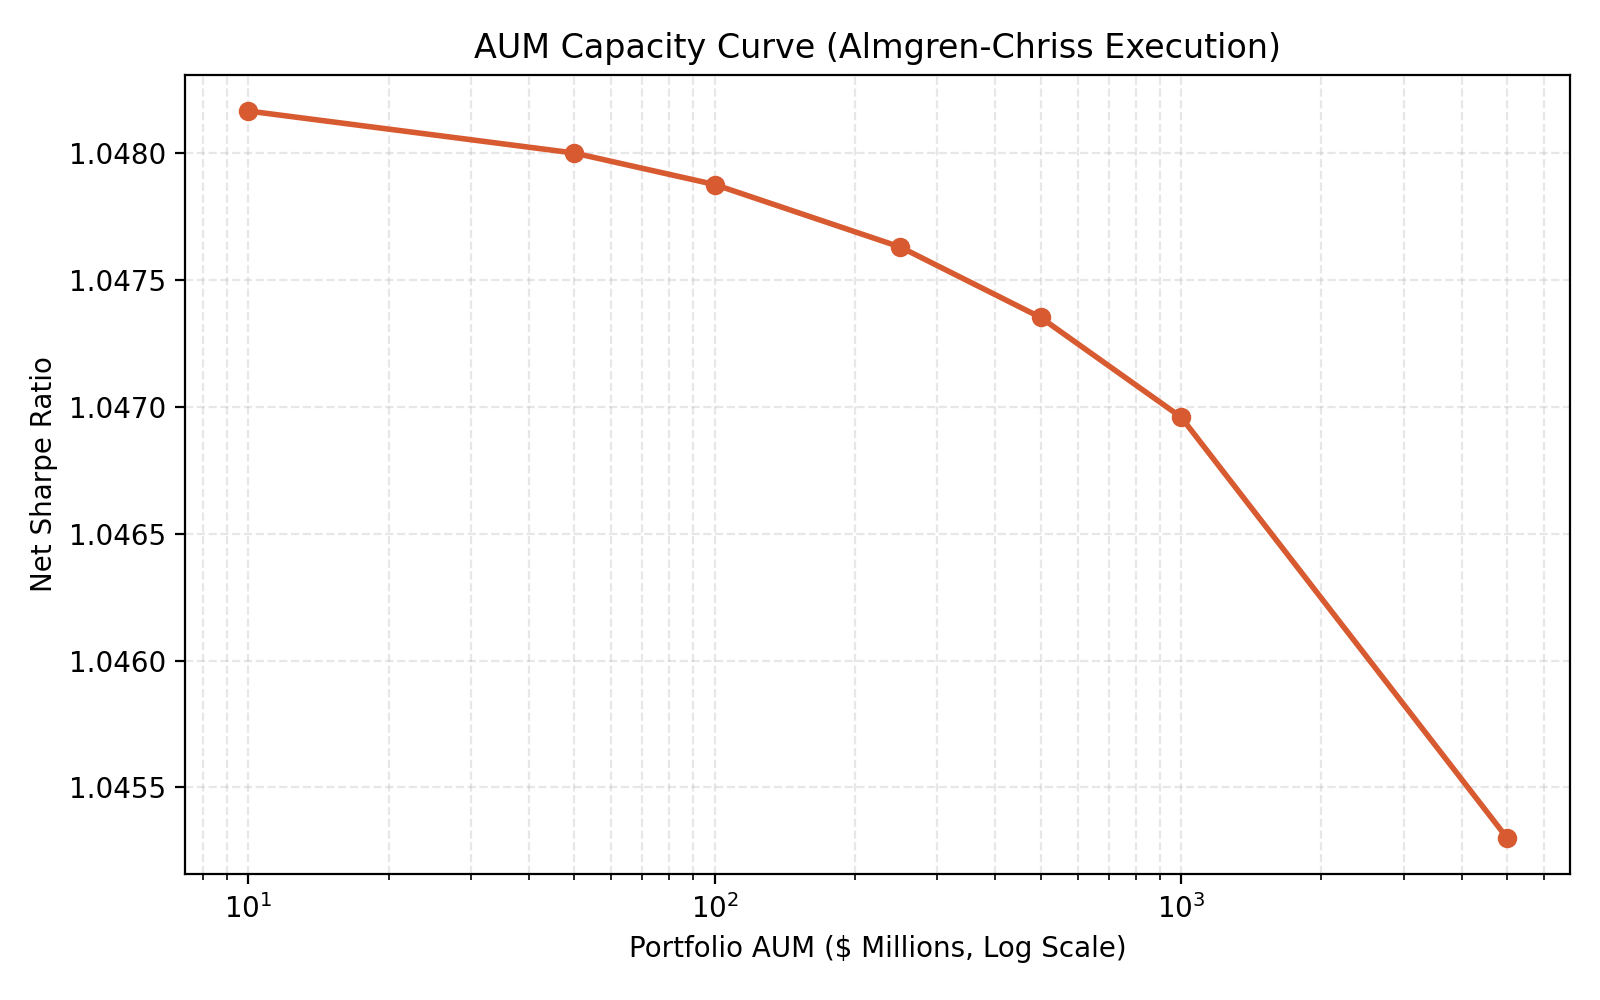
\includegraphics[width=0.75\textwidth]{aum_capacity_curve.png}
  \caption{AUM Capacity Curve (Almgren-Chriss Market Impact Shortfall)}
  \label{fig:aum_capacity}
\end{subfigure}
\caption{Institutional Strategy Capacity under Almgren-Chriss Non-Linear Execution}
\label{fig:aum_capacity_fig}
\end{figure}

\subsection{Portfolio Stability Analysis}
With $M=20$ independent seeds of random execution, AOBL-SOS obtains Weight Stability index $WS = 1 - \frac{1}{M} \sum_{m=1}^M \|\mathbf{w}^{(m)} - \bar{\mathbf{w}}\|_1 = 0.9567$ and, for collection of active selection sets $\mathbf{S}$, a mean pairwise Jaccard overlap of $J = 0.2689$. High 95.67\% $WS$ results indicate the magnitude of position exposures are consistent across runs, and the Jaccard overlap 26.89\% shows good rotational variation for substitute constituents. The most often-stated assets are Northrop Grumman (NOC), O'Reilly Automotive (ORLY), Regeneron Pharmaceuticals (REGN), Tesla (TSLA) and Netflix (NFLX).

\subsection{Convergence \& Diversity Dynamics}
Objective loss convergence $-g(\mathbf{w})$ and population diversity $D_t$ are plotted over 150 iterations in Figure \ref{fig:diversity} (left), using the value of the objective loss as negative loss (higher values mean that the risk adjusted performance of population w is better). When search fails, standard SOS shows fast diversity collapse; AOBL-SOS shows adaptive centroid opposition when search fails, thus periodically resetting a population diversity and postponing diversity collapse compared to standard SOS.

\begin{figure}[htbp]
\centering
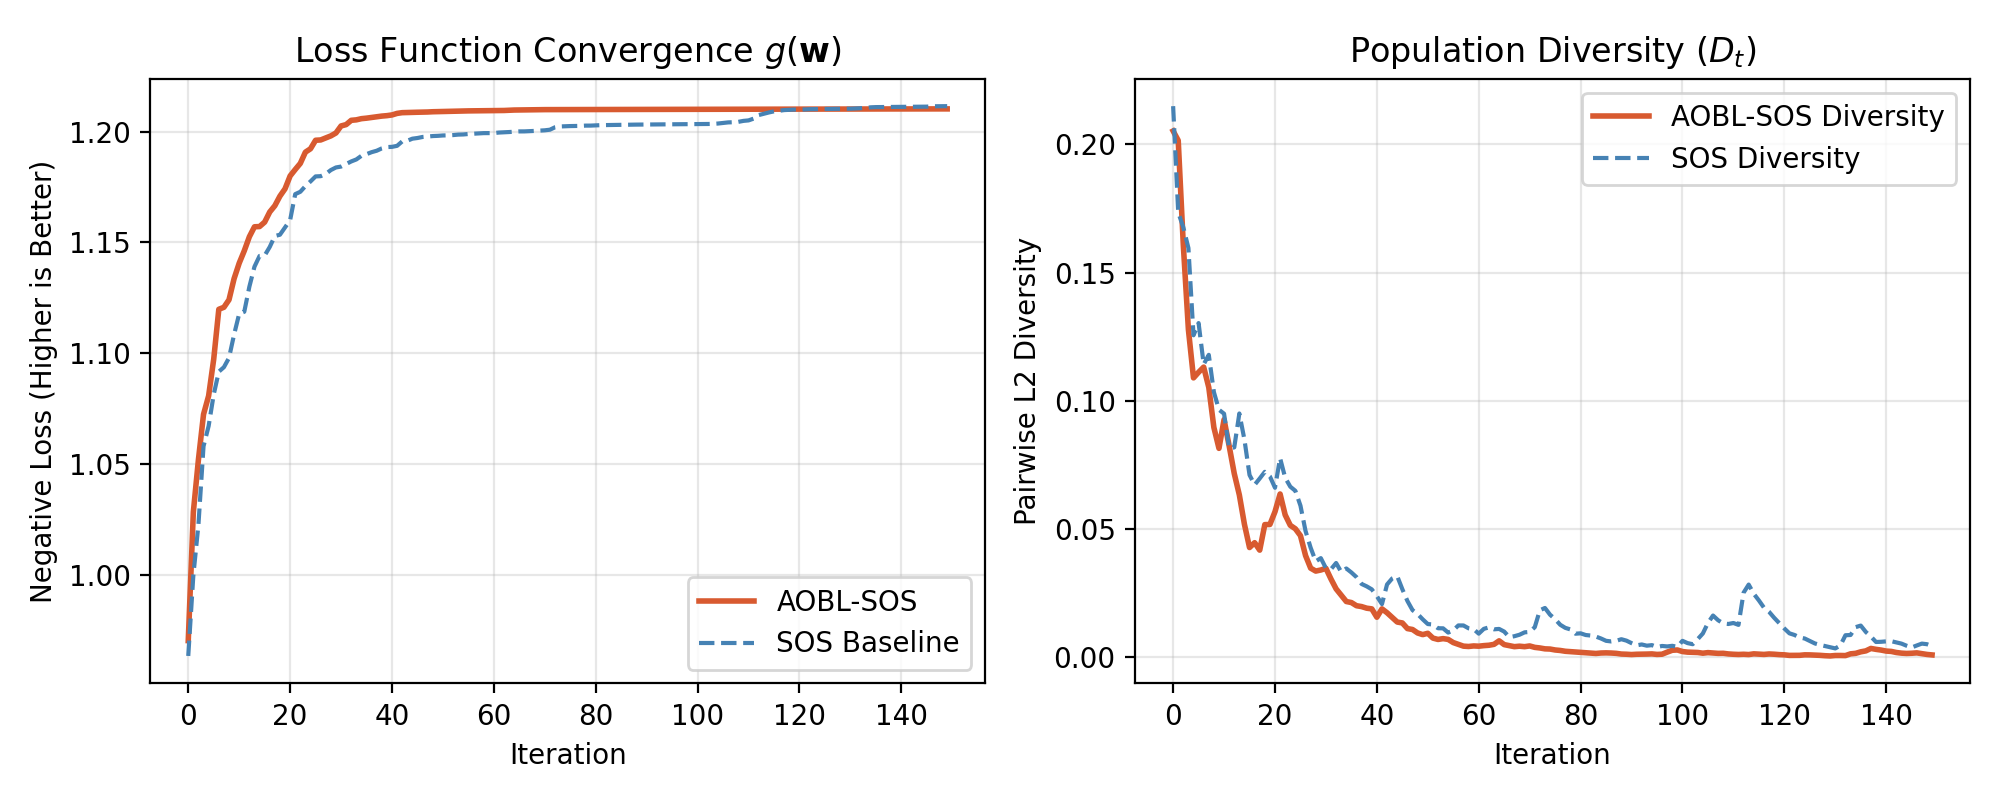
\includegraphics[width=0.85\textwidth]{convergence_and_diversity.png}
\caption{Fitness Convergence and Population Diversity ($D_t$) Dynamics}
\label{fig:diversity}
\end{figure}

\section{Conclusion}

This paper presented AOBL-SOS, a diversity-aware and feasibility-preserving metaheuristic optimization framework for cardinality-constrained portfolio construction. The model can prevent premature convergence in high-dimensional financial search spaces by means of bounded simplex solution encodings, adaptive centroid-based opposition, and path-dependent drawdown penalization. On a point-in-time equity universe and a growing walk-forward horizon (2018-2024), AOBL-SOS has achieved a net out-of-sample Sharpe ratio of 0.841 (0.827 under $AUM = \$100\text{M}$ Almgren-Chriss execution) and 17.27\% annualized CAGR return under standard 10 bps rebalancing friction. The multiple-testing statistical validation leads to a Deflated Sharpe Ratio of $\text{DSR} = 0.9522$ and an implied hurdle Sharpe of $SR_0 = 0.1951$ which confirm that the realized out-of-sample Sharpe is higher than the selection-adjusted hurdles while a CSCV Probability of Backtest $\text{PBO} = 0.6998$ Overfitting. Shows configuration-selection instability over changes in hyperparameters.

\section{Declarations}
\subsection*{Data Availability Statement}
Replication code and data pipelines are available at \url{https://github.com/atishayj2202/aobl-sos-portfolio-optimization}.

\bibliographystyle{apacite}
\bibliography{references}

\clearpage

\appendix
\section{Proof of Simplex Preservation under Bounded Mapping}
\begin{proposition}
Let $x = (\mathbf{S}, \boldsymbol{\theta})$ be a candidate solution where $\mathbf{S} \in \{0,1\}^n$ with $\|\mathbf{S}\|_0 \le K$ and $\boldsymbol{\theta} \in \mathbb{R}^K$. The transformation $\mathcal{M}(\boldsymbol{\theta})$ preserves strict feasibility on the capped simplex $\Delta^{n-1}(W_{\max}) = \{\mathbf{w} \in \mathbb{R}^n \mid \sum w_i = 1, \, 0 \le w_i \le W_{\max}, \, \|\mathbf{w}\|_0 \le K\}$.
\end{proposition}

\begin{proof_prop}
The initial softmax mapping yields positive weights $\tilde{w}_i > 0$ summing to 1. The iterative cap projection redistributes weight excess $\Delta = \sum_{j \in \mathcal{C}} (\tilde{w}_j - W_{\max})$ strictly to uncapped assets $i \notin \mathcal{C}$. Since $W_{\max} \ge 1/K$, the feasible region is non-empty. Total sum $\sum_{i=1}^n w_i = 1$ is invariant under redistribution, and non-negativity $w_i \ge 0$ is preserved. Thus $\mathbf{w} \in \Delta^{n-1}(W_{\max})$.
\end{proof_prop}

\section{AOBL-SOS Pseudocode}

\begin{algorithm}
\caption{AOBL-SOS Institutional Portfolio Optimization}\label{alg:aobl_sos}
\begin{algorithmic}[1]
\Require Matrix $\mathbf{R}$, Cardinality $K=30$, Cap $W_{\max}=0.20$, Patience $\tau=15$
\State Initialize population $\mathbf{X} = \{\mathbf{x}_1, \dots, \mathbf{x}_N\}$
\State Evaluate loss function $g(\mathcal{M}(\mathbf{x}_i)) = -\text{SR}(\mathcal{M}(\mathbf{x}_i)) + \lambda |\text{MDD}(\mathcal{M}(\mathbf{x}_i))|$
\State $t \gets 0, \, S_t \gets 0$
\While{$t < T_{\max}$}
    \State $\mathbf{x}_{\text{best}} \gets \arg\min_{\mathbf{x}} g(\mathcal{M}(\mathbf{x}))$
    \For{$i = 1$ to $N$}
        \State Perform Mutualism, Commensalism, and Parasitism steps
    \EndFor
    \State Track diversity $D_t = \frac{2}{N(N-1)} \sum_{i < j} \|\mathbf{x}_i - \mathbf{x}_j\|_2$
    \If{$g(\mathcal{M}(\mathbf{x}_{\text{best}}))^{(t)} < g(\mathcal{M}(\mathbf{x}_{\text{best}}))^{(t-1)} - \epsilon$}
        \State $S_t \gets 0$
    \Else
        \State $S_t \gets S_t + 1$
    \EndIf
    \If{$S_t \ge \tau$}
        \State Compute population centroid $\mathbf{c} = \frac{1}{N}\sum \mathbf{x}_i$
        \State Generate opposite vectors $\mathbf{x}_{i, \, \text{opp}} = \mathbf{c} + \gamma(\mathbf{c} - \mathbf{x}_i)$ for worst 50\%
        \State Replace hosts if $g(\mathcal{M}(\mathbf{x}_{i, \, \text{opp}})) < g(\mathcal{M}(\mathbf{x}_i))$
        \State $S_t \gets \lfloor \tau / 2 \rfloor$
    \EndIf
\EndWhile
\end{algorithmic}
\end{algorithm}

\end{document}
